% Chapter 2

\chapter{Navigation Among Movable Obstacles: state of the art} % Main chapter title

\label{Chapter2} % For referencing the chapter elsewhere, use \ref{Chapter2}

\section{Determining appropriate comparison criteria}

\paragraph{} As a synthesis of the diversity of NAMO definitions accross publications, we summarize NAMO as the problem of having an autonomous agent that navigates in an environment, going from its initial pose to a goal pose, while being authorized to move obstacles in order to reach the goal at a lower cost (in terms of time, distance or energy consumption, generally). The many approaches to the problem and their contexts highlight a need to characterize them, thus our establishing comparison criteria.

\paragraph{} We propose to divide these comparison criteria into three main categories: hypotheses, approaches and performance criteria. These criteria have been established according to the actual content of the studied articles and the goal we have set for ourselves to bring social and dynamic considerations.

\subsection{Hypotheses}

\begin{itemize}
  \item \textbf{Knowledge of the environment} The most significant criterion to understand the context of a navigation algorithm is "what does the robot know about the environment?". This includes the way it represents it (metric/topologic map, dimensions, \dots) and how much the robot knows of it at the moment of the algorithm's execution (none, partial or complete knowledge). If the knowledge is not complete, this criterion also includes hypotheses on the unknown environment (e.g., can the robot consider it free space, or obstacle-occupied space?). All the papers presented in the following pages provide this information.
  \item \textbf{Obstacle characteristics} The nature, shape, cinematic or frictional constraints, associated semantics (physical characteristics like center of gravity, weight, moment of inertia, \dots), autonomous movement or not of the considered obstacles all condition the final algorithm proposition, because these characteristics partly define the problem solution space (e.g., poses where to put an object may differ whether we represent it as a rectangle or a polygon, cinematic or frictional constraints may reduce the manipulation possibilities, \dots).
  \item \textbf{Robot characteristics} Naturally, in the same way an algorithm depends on the suppositions we make on obstacles, it also depends on the ones we make on the robot itself. When a specific robot is used, it is important to know its manipulation capabilities (only pushes? translations only? rotation?), its geometric representation, its navigation capabilities (differential drive that only allows translation XOR rotation? Omnidirectional drive that allows both at the same time?), but also its sensing capabilities (on-board sensors like cameras or sonars, and their effective range). By comparing the requirements for the robot in a proposition, we can know if it will be applicable with our Pepper robot or not.
  \item \textbf{Problem class} In his first paper \parencite{stilman_navigation_2005} published in 2005, Dr. Stilman, the founder of the NAMO domain, established a NAMO problem classification inspired from an existing one in the field of rearrangement planning \parencite{ben-shahar_practical_1998}. The $LP$ notation is for "Linear Problem". A NAMO problem has a linear solution when there exists a sequence of free space (areas were the robot can move without entering in collision with obstacles) components such that merging two adjacent components does not constrain the merge of the following adjacent components. The $k$ notation in $LP_k$ relates to the maximal number of obstacles the algorithm should consider when trying to independently connect two disconnected components of free-space. Independently means that the algorithm operates under the assumption that moving $k$ obstacles to create this connection will not affect the solvability of following solutions. $k$ therefore characterizes the exponential complexity of a NAMO problem, since it means that we consider every manipulation combinations for $k$ obstacles when evaluating a connection plan. For example, a situation where two adjacent rooms are linked together through a single door, and a single obstacle is present in the doorway, then the problem class of navigating to the other room is $LP_1$. If it were necessary to move two obstacles from the doorway to go to the other room, the problem class would be $LP_2$. The notation is further explained and refined in another paper \parencite{stilman_planning_2008} published in 2008. This notation allows us to quickly know what kind of situation an algorithm will be able to solve or not.
\end{itemize}

\subsection{Approaches}

\begin{itemize}
  \item \textbf{Path Planning Algorithm(s) and heuristics} The NAMO algorithms in the considered papers are systematically building upon existing graph search algorithms like A* or Dijkstra\footnote{Basic presentation \url{http://theory.stanford.edu/~amitp/GameProgramming/AStarComparison.html}}, or use them as path finding subroutines. Often, as is the case when using A*, heuristics are used to direct the search and obtain gains in terms computer time performance. Knowing on which algorithm and heuristics the new proposition is built upon is essential to characterize it, and judge whether it is appropriate for our own proposition.
  \item \textbf{Evaluation and evolution of an obstacle's "movable" characteristic and its associated cost} The way the different algorithms take movable obstacles into account differs from one algorithm to the other. Some propositions depend on knowing beforehand whether an obstacle is actually tagged as movable or not, while others deduce this status on-line (i.e while navigating). Some use a constant cost for manipulating all obstacles, while others compute a cost according to known physical properties of the obstacle, like its weight. Knowing what a proposition is using to compute the cost of manipulating an obstacle is essential to understand its limitations.
  \item \textbf{Object manipulation maneuver planning} The way the proposition has the robot place itself by the obstacle for manipulation matters too. Whether it is only based on geometric considerations or cinematic ones on the obstacle or the robot. Whether the algorithm is or is not capable of reconsidering its placement next to the obstacle depending on new geometric or cinematic information that is collected during the navigation execution also affects the algorithm proposition.
  \item \textbf{Planning taking uncertainty into account} A real world setting, using a real robot, implies limited sensing and actuation capabilities, and therefore, uncertainty about the state of the environment and the robot. Since our long-term goal is to apply our proposition to real-world situations, it is important to take note of the many different strategies used to take uncertainty into account.
\end{itemize}

\subsection{Performance criteria}

\begin{itemize}
  \item \textbf{Evaluation in a simulated/real setting} In robotics, it is paramount to know whether an algorithmic proposition has made it to the stage of real-world experimentation or not. Since it is a field that is heavily anchored in reality, an experimental validation in a real-world setting is far more valuable than a simulation.
  \item \textbf{Computation time} In robotics, algorithms that can be executed in a short time span are very valuable, since it is a world of real-time computation and actuation. If computing a new plan were to take more time than it would to execute it, it would arguably be considered too expensive. Thus, knowing if a proposition is executable in real-time or not matters a lot.
  \item \textbf{Optimality and completeness} For about any algorithm, knowing whether it is complete (always return a solution when there is one) and guaranteed to be optimal (the returned solution is always the best) matters. In a context where the robot must make decisions upon partial knowledge on the environment, an algorithm is considered \textit{locally optimal} if it is guaranteed to return the best solution given its current belief state of the environment.
  \item \textbf{Optimality target} Even if an algorithm can not guarantee optimality, it will still try to optimize a certain cost. The type of cost an algorithm can manage is also a significant criterion, since in the context of robotics many types of cost are used: distance, time, energy, risk, \dots
  \item \textbf{Social acceptability} This criterion does not come from the reading of our corpus but from the goal we have set for ourselves to seek if there are any social acceptability considerations in existing NAMO algorithms. It is thus interesting to our research to see to what extent the existing propositions care for social problematics or not.
  \item \textbf{Number and Density of obstacles} Since NAMO computations depend on each and every individual obstacle, it makes sense that the number and repartition of obstacles in the environement would affect the computation efficiency of an algorithm. Knowing the maximum values with which algorithms have been successfully tested in real-time conditions, for example, would allow us to compare the efficiency of the different algorithms.
\end{itemize}

\subsection{Recapitulative tables}

\begin{figure}[H]
\centering
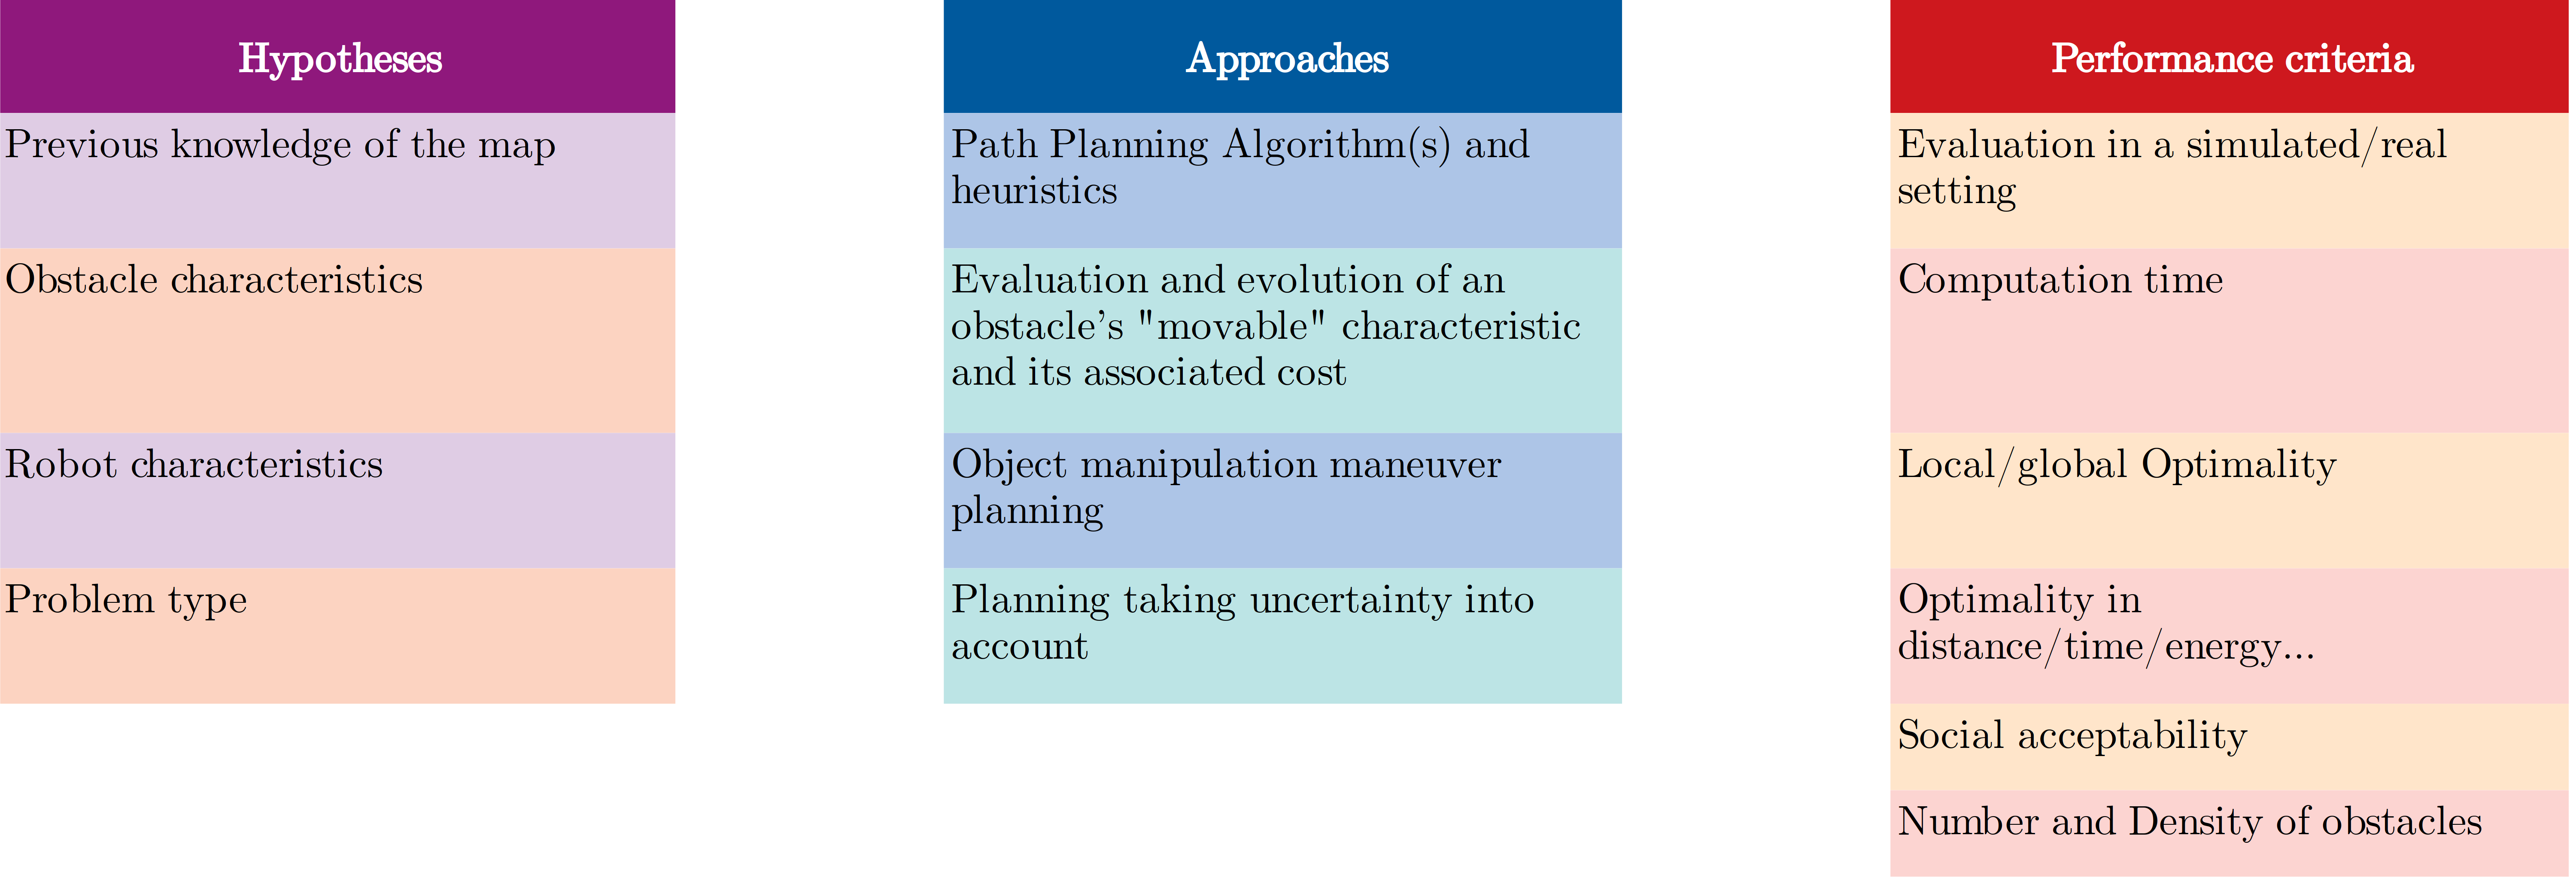
\includegraphics[width=13cm]{Comparison_Table/01_comparison_criteria}
\decoRule
\caption[Comparison criteria listing]{Comparison criteria, sorted by type.}
\label{fig:comparison_criteria}
\end{figure}

\clearpage

\section{Comparison and cross-comparison}

\subsection{Comparison Tables}

\paragraph{} In order to be able to properly situate our work in the context of the currently available research in the NAMO domain, we have made several comparison tables according to the criteria presented beforehand. In the following pages, you will find the booleanized comparison tables, where each global criteria is divided into boolean sub-criteria that the paper answers to or not. The detailed comparison and cross-comparison tables are available in the \nameref{comparison_tables} Appendix. Abbreviations are explained in the detailed comparison table.

\paragraph{} Emphasized and bold cells with the "[Prop]" reference are criteria that are validated by the final proposition we make in Chapter \ref{Chapter4}.

\begin{figure}[H]
\centering
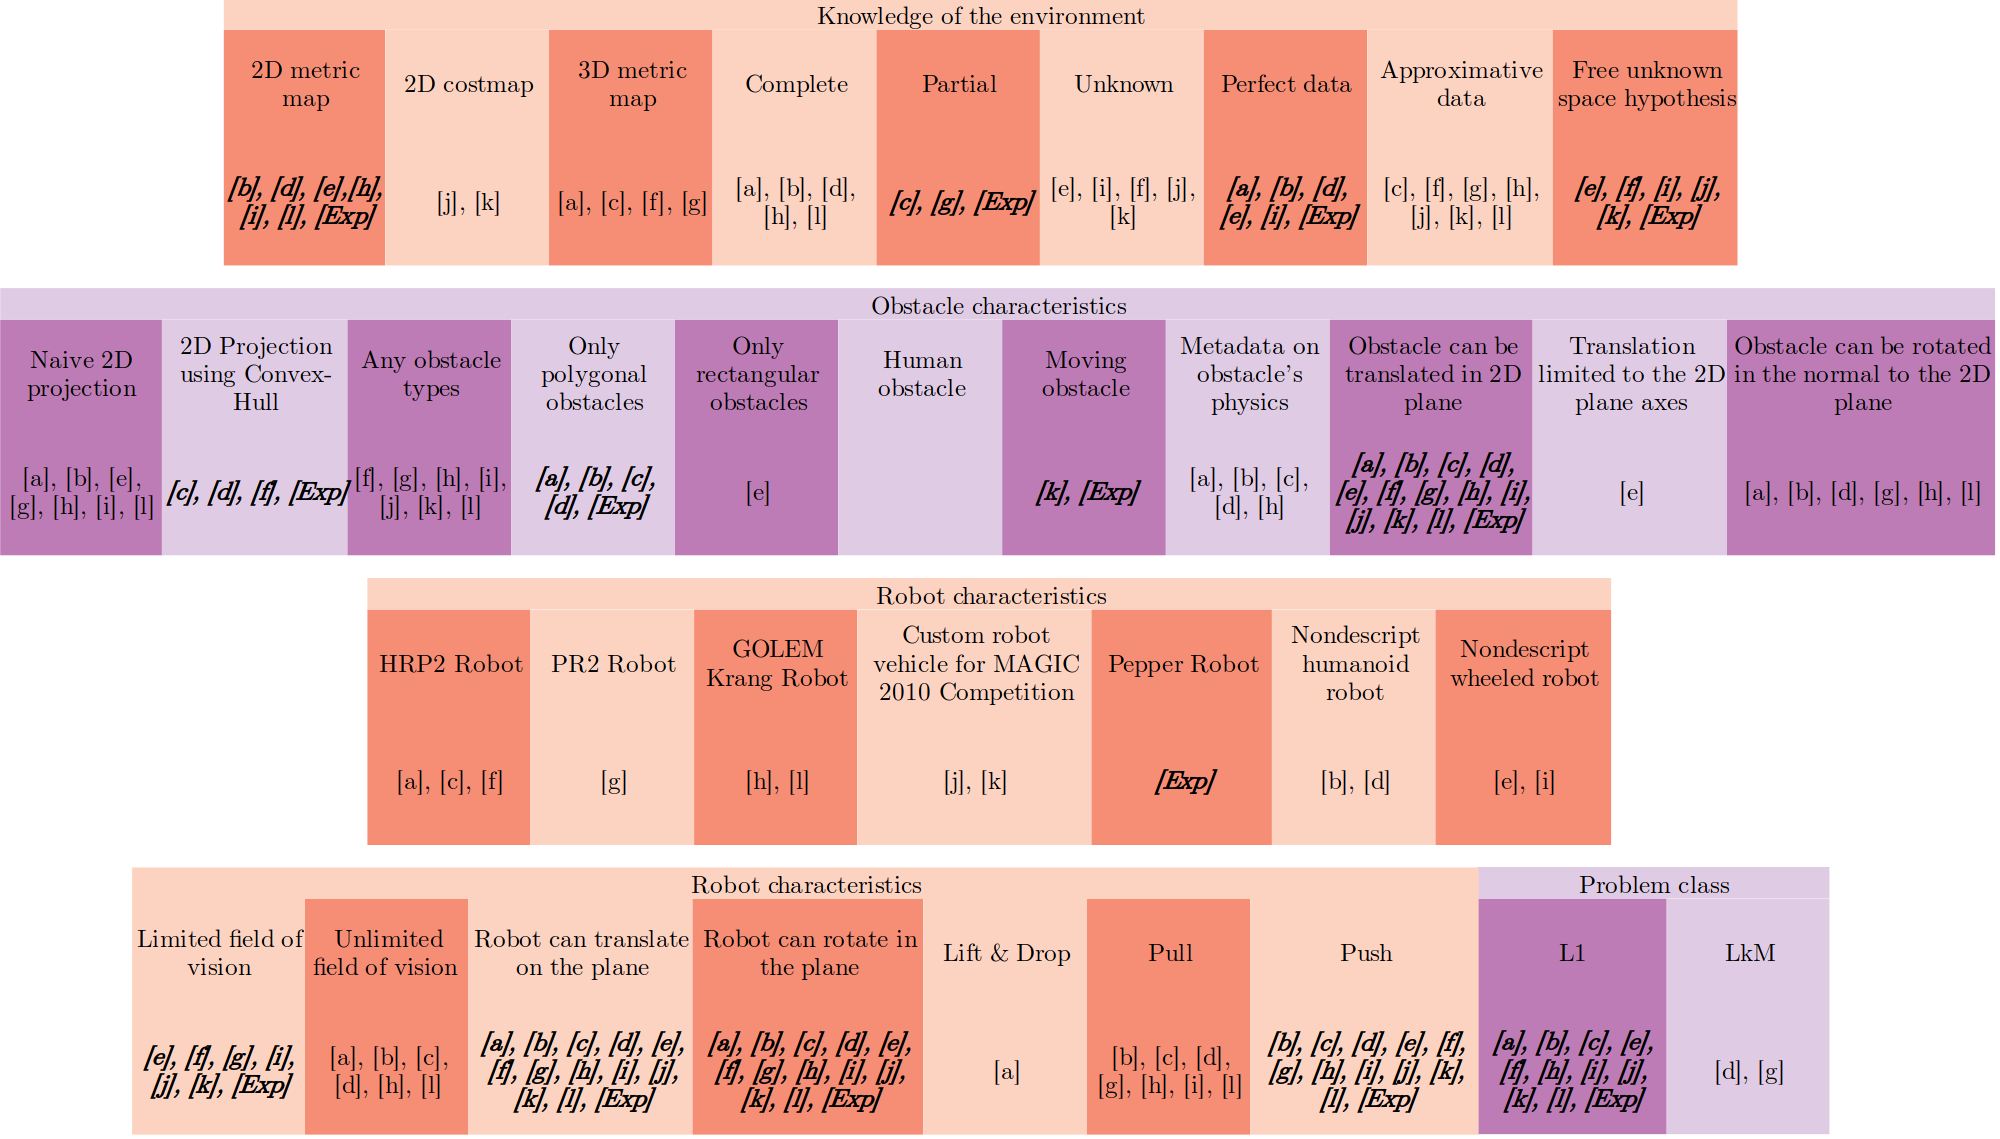
\includegraphics[width=\linewidth]{Comparison_Table/a_hypotheses}
\decoRule
\caption[Hypotheses comparison tables]{Hypotheses comparison tables}
\label{fig:hypotheses_comparison_tables}
\end{figure}

\begin{figure}[H]
\centering
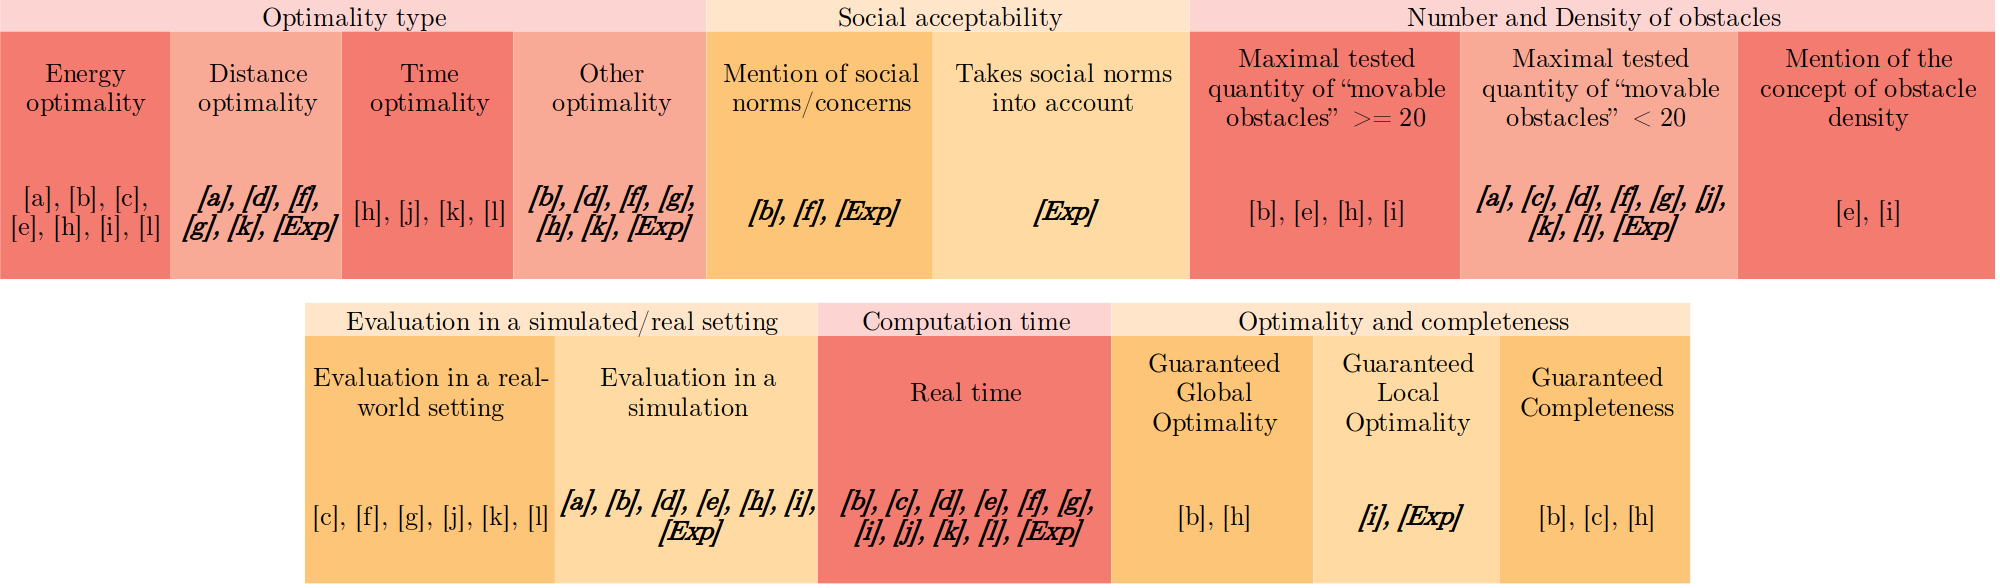
\includegraphics[width=\linewidth]{Comparison_Table/c_performance}
\decoRule
\caption[Performance criteria comparison tables]{Performance criteria comparison tables}
\label{fig:performance_comparison_tables}
\end{figure}

\begin{figure}[H]
\centering
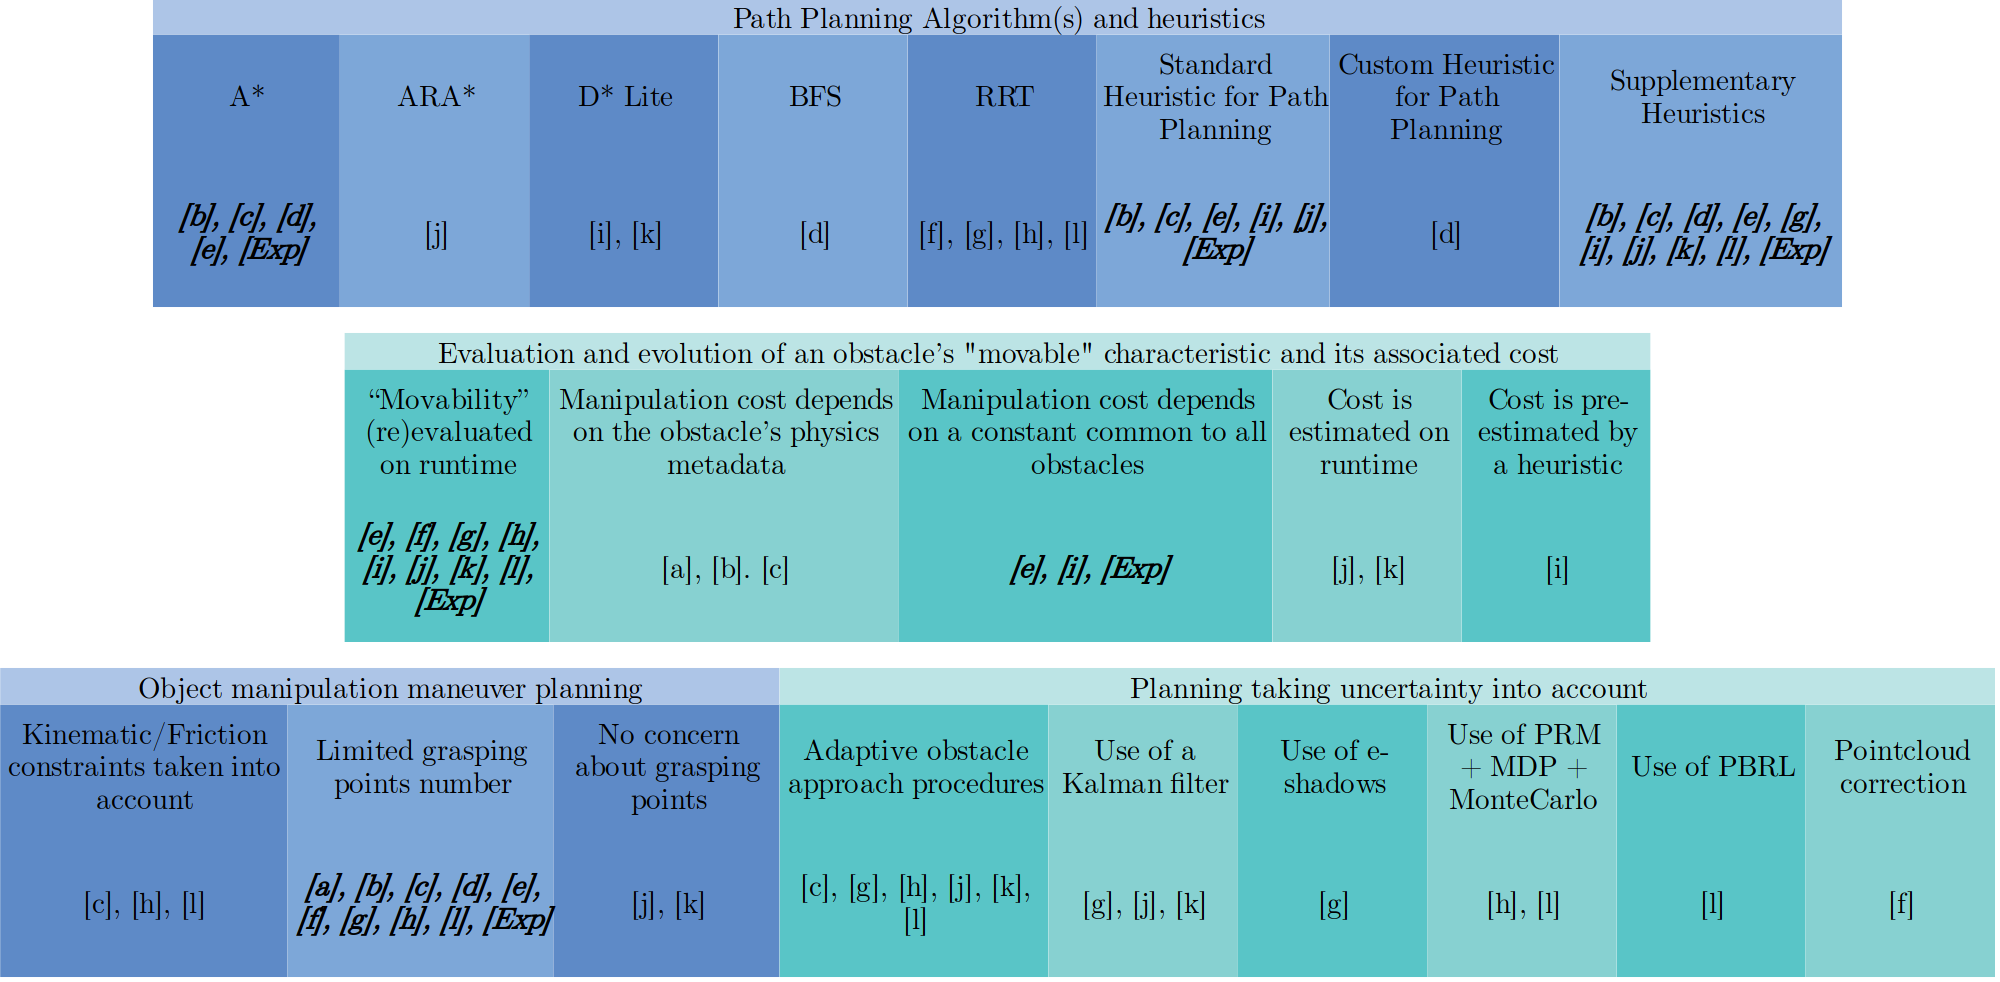
\includegraphics[width=\linewidth]{Comparison_Table/b_approaches}
\decoRule
\caption[Approaches comparison tables]{Approaches comparison tables}
\label{fig:approaches_comparison_tables}
\end{figure}

\subsection{Analysis}

\paragraph{} The first remark we can draw from our tables is that while there is a wide diversity of propositions to solve the problem of Navigation Among Movable Obstacles, and each proposition is only applicable in a well-defined context, there are quite a few common points. For example, in Figure \ref{fig:hypotheses_comparison_tables}, the Obstacle characteristics and Robot characteristics tables show that as long as the robot is not manipulating an obstacle, its freedom of movement is not limited to specific translation or rotation movements. The main reason why the movement of the robot when manipulating obstacle is often limited from the get-go, reducing the action space, is because it also reduces the search space of the algorithm, thus reducing the computation time complexity \parencite{stilman_navigation_2005}.

\paragraph{} As many of the papers \parencite{stilman_navigation_2005, stilman_planning_2007, stilman_planning_2008, wu_navigation_2010, levihn_planning_2013, levihn_locally_2014, scholz_navigation_2016} recall it, the complexity of the NAMO problem would quickly be untractacle if we were to consider any manipulation on every obstacle in the environment to find a path to the goal: it has been shown by Wilfong that even a simplified variant of the domain where the final positions of the obstacles in a polygonal environment are specified by the user (which is closer to the domain of rearrangement planning), finding the obstacle configuration that allows to reach the goal in the best way is a P-Space Hard Problem \parencite{wilfong_motion_1991}. The same work shows that if the final positions of the obstacles are not known, then the problem becomes NP-hard. A more recent work by Demaine et. al. showed that if we only considered push actions in a planar grid (problem analogous to the game of Sokoban\footnote{Wikipedia page on Sokoban: \url{https://en.wikipedia.org/wiki/Sokoban}}), the problem is NP-complete. Stilman summarizes this by concluding that "The size of the search space is exponential in the number of movable objects. Furthermore, the branching factor of forward search is linear in the number of all possible world interactions" \parencite{stilman_planning_2008}. Further discussion on the complexity of the domain with illustrations can be found in Stilman's thesis on NAMO \parencite{stilman_navigation_2007}.This is why the robots are often limited to push or pull actions, following a translation movement in a single direction in the propositions. When it is not so, like in \parencite{okada_environment_2004}, it is because only the nearest obstacle poses to the robot are considered (making the proposition non-optimal), and no real-time constraint is given. Actually, among all the selected papers, this is the only one that does not guarantee or show results of real-time execution.

\paragraph{} Another important reason that can motivate the reduction of the action space of the robot is the will to reduce the risk of manipulating obstacles in an unexpected way. Indeed, grasping an obstacle in order to pull or pick \& place it augments the number of interactions with the environment, and with that, the chance that something might go wrong: especially, as is mentioned in \parencite{stilman_planning_2007}, the robot might lose its balance.

\paragraph{} Figure \ref{fig:hypotheses_comparison_tables} (Robot Characteristics table) also shows that a diversity of real and simulated robots have been used for experimenting with NAMO algorithms, but it is to be noted that the ones that were actually used for a real world experiment are very costly robots (PR2\footnote{PR2 Characteristics: http://www.willowgarage.com/pages/pr2/specs}, HRP2\footnote{HRP2 Characteristics: http://global.kawada.jp/mechatronics/hrp2.html} and GOLEM\footnote{GOLEM Characteristics: http://www.golems.org/projects/krang.html}) at the exception of the custom robotic platform built by Clingerman \parencite{clingerman_estimating_2014}. However, the robot used by Clingerman is arguably not capable of handling problems as complex as the propositions of Stilman and Levihn, since it does not have a manipulation arm.

\paragraph{} Figure \ref{fig:approaches_comparison_tables} (Path Planning Algorithm(s) and heuristics Table) confirms that all propositions are built upon a variety of existing path finding algorithms. In most papers, the choice of the path finding algorithm they build upon is not explicitly justified. The only one that justifies the choice of its Path Finding algorithm is Clingerman \parencite{clingerman_dynamic_2015}, since it allows him to potentially manage autonomously moving obstacles, since it is based off the D* Lite algorithm (see \parencite{koenig_fast_2005} and\footnote{Koenig's other paper on D* Lite: \url{http://idm-lab.org/bib/abstracts/papers/aaai02b.pdf}}), but no experiment with a changing environment is shown. Almost all papers use some sort of heuristic, either for the path finding subroutine or choosing which obstacle to evaluate, and some of these heuristics come at the cost of optimality \parencite{stilman_navigation_2005, wu_navigation_2010}. Some papers \parencite{stilman_planning_2007, levihn_foresight_2013, levihn_planning_2013, clingerman_estimating_2014, clingerman_dynamic_2015, scholz_navigation_2016} offer means to take uncertainty into account. All of them have adaptive approach procedures that are executed when nearing the obstacle, but some use much more elaborate approaches to this end, like using probabilistic models \parencite{levihn_planning_2013, scholz_navigation_2016}.

\paragraph{} It is noteworthy that many of the algorithms do not focus on guaranteeing the optimality of the plans they produce, or even their completeness. This can easily be explained by the fact that, in robotics, real-time performance is paramount, and trading off optimality for performance is often prefered. However, sensible approaches like \parencite{stilman_navigation_2005, wu_navigation_2010}, where the proposition contains an original algorithm that is optimal, but also a modified version that improves performance at the cost of optimality, are more interesting, as it is often easier to improve the computational performance of an algorithm by sacrificing its optimality, than trying to make a non-optimal algorithm optimal.

\paragraph{} In the selected papers, about half make propositions to deal with an unkwown or partially known environment (which is definitely correlated with the fact that the robot is considered to have a limited field of vision), and it could give the impression that this is a well-treated subset of NAMO problems. However, this is in fact related to our initial bias that we want to build a solution that can manage a partially known environment. In addition to the selected papers, quite a few of other briefly examined papers strongly related to NAMO \parencite{chen_practical_1991, okada_humanoid_2005, nieuwenhuisen_effective_2008, berg_path_2009, kaelbling_hierarchical_2011, levihn_hierarchical_2013, levihn_autonomous_2014} rely on a complete knowledge of the environment, and also, perfect data (that is, they assume that what the robot knows of the environment is always almost perfectly like the real setting). It is the paper of Kakiuchi et.al. \parencite{kakiuchi_working_2010} that brought the first extension to NAMO in unknown environments \parencite{levihn_locally_2014} but as it was only a local approach (the robot only reacts to a specific movable obstacle, without considering all the others in the computation of the new plan) it had no hopes of optimality. Wu and Levihn were the ones to formulate a locally optimal algorithm for NAMO in completely unknown environments \parencite{wu_navigation_2010, levihn_locally_2014}. Levihn and Stilman then worked on another approach for partially known environments that does not guarantee optimality, but improves performance and allows for greater complexity in obstacle configurations and robot action set \parencite{levihn_foresight_2013}. Clingerman also proposed later another solution for NAMO in unknown environments \parencite{clingerman_estimating_2014, clingerman_dynamic_2015}, however this solution does not consider the manipulation of an obstacle as an action in itself and simply makes the robot try to "pass through" the obstacle, without trying to consider if it is going to collide with its environment.

\paragraph{} Finally, it is to be noted that none of the selected papers (and also the ones that were only briefly examined) consider a case with movable obstacles mixed with humans (Figure \ref{fig:hypotheses_comparison_tables}, Obstacle characteristics). Also, if Stilman \parencite{stilman_navigation_2005} and Kakiuchi \parencite{kakiuchi_working_2010} briefly mention the necessity to consider the frailty of a manipulated obstacle, which can be interpreted as taking social conventions into account, neither them or any other paper actually try to adapt their NAMO algorithm to social conventions or norms.

\subsection{Situating our work in the established context}

\paragraph{} In the end, we chose to base our following work on the solution proposed by Wu and improved by Levihn \parencite{wu_navigation_2010, levihn_locally_2014}, because:
\begin{itemize}
  \item It is a solution designed for unknown environments, thus also adapted to partially known ones,
  \item One of our initial objectives was for our proposition to make optimal decisions: their solution is the only one allowing that for partially known environments,
  \item The reduction to push actions is not a problem for us since we did not want to spend time on grasping problematics in the first place (this could have been a lot of time, since grasping problematics have their very own research field \parencite{sahbani_overview_2012}), and the grasping capabilities of Pepper are very limited (low applied force in particular).
\end{itemize}

\paragraph{} The next chapter will therefore thoroughly present the solution proposed by Wu et. al. \parencite{wu_navigation_2010}, and apply the improvements proposed by \parencite{levihn_locally_2014}. Then, we will be able to bring our own propositions.
